% Report skeleton for CS-E4780 (ACM proceedings template, 4-5 pages).
%
% Headings and figure slots only. The course requires that you write the text yourselves:
% the analysis, the interpretation of results and the conclusions. Each section has a comment
% listing what the grading criteria look for and where the supporting evidence is in the repo.
% Delete the comments as you go. Upload to Overleaf ("ACM Conference Proceedings" template) or
% compile locally with: latexmk -pdf skeleton.tex
\documentclass[sigconf,nonacm]{acmart}
\usepackage{graphicx}
\graphicspath{{../results/figures/}{../docs/}}

\title{Detecting Trading Trends in Financial Tick Data}
\subtitle{CS-E4780 Scalable Systems and Data Management Course Project}

\author{Name Surname}
\affiliation{\institution{Aalto University}\city{Espoo}\country{Finland}}
\email{first.last@aalto.fi}
\author{Name Surname}
\affiliation{\institution{Aalto University}\city{Espoo}\country{Finland}}
\email{first.last@aalto.fi}

\begin{document}

\begin{abstract}
% One paragraph: problem, approach (Kafka + Flink, 5-min tumbling windows, EMA38/EMA100,
% crossover advisories), the headline results (correctness, throughput, scaling, latency).
\end{abstract}

\maketitle

\section{Introduction}
% Background (tick data, why EMAs/crossovers), the two queries and the visualization,
% the dataset (cite Frischbier et al. 2022), what the report contains.

\section{Dataset Analysis}
% Rubric ("Academic writing: strong focus on dataset analysis", "handling of long-tail
% distributions"). Evidence: analysis/longtail.py (figure longtail-week.png), analysis/load_day.py,
% clocks.py, late_check.py (out-of-order and placeholder trades), event-type shares per exchange.
% \begin{figure}[t]\includegraphics[width=\linewidth]{longtail-week}\caption{...}\end{figure}

\section{System Architecture}
% Rubric: design for real-time processing, complex event processing, metadata handling,
% normalization, scalability. Design choices to describe and justify:
%  - Kafka topic keyed by symbol (per-symbol order, partitioning), 8 partitions
%  - event-time windows, per-partition watermarks, out-of-order bound, idleness, end-of-stream marker
%  - keyBy(symbol) for windows and EMA state (what state is kept, why it is small)
%  - event classification (trades / quotes and housekeeping / placeholder times / malformed)
%  - subscriptions: compute all symbols, publish for a subset
%  - late trades to a side output instead of silent loss
%  - alternatives considered and why rejected (e.g. sliding windows, processing time,
%    per-event EMA, checkpointing on or off)
% Architecture figure: redraw it (the mermaid diagram in the README is a starting point; the
% old "Streaming Pipeline Architecture Flowchart.png" in dashboard/ predates these changes).

\section{Implementation}
% Rubric: event handling, windowing and EMA state, crossover detection, normalization,
% metadata usage; hardware/cloud services, programming tools, GUI tools.
%  - Producer (Python, confluent-kafka), message format, pacing
%  - Flink job classes (TickParser, EventRouter, LastTradeAggregate, EmaProcessor)
%  - Tie-breaking rule for the window close, first-window behaviour (EMA_0 = 0)
%  - Docker images and compose setup, dashboard (Streamlit + Altair)
%  - Reference implementation and validator (pandas)

\section{Performance Evaluation}
\subsection{Setup}
% Hardware (MacBook Air M5: cores, memory), Docker Desktop CPUs/memory, software versions,
% dataset portion used, number of repeats. Limitations (passively cooled laptop,
% performance vs efficiency cores, producer and broker on the same machine).

\subsection{Correctness}
% results/scalability/<run>/validation.json (full week vs answer key) and the OOO sweep.
% The Docker demo checks itself the same way on any machine (docs/TESTING.md), and CI runs it on every push.

\subsection{Throughput and Scalability}
% results/figures/scalability-throughput.png, scalability-cpu.png, results/summary.md tables.
% Per-exchange runs and event types (EVENTS=all): experiments/run_remaining.sh, then the
% "Scalability across runs" table in results/summary.md.
% \begin{figure}[t]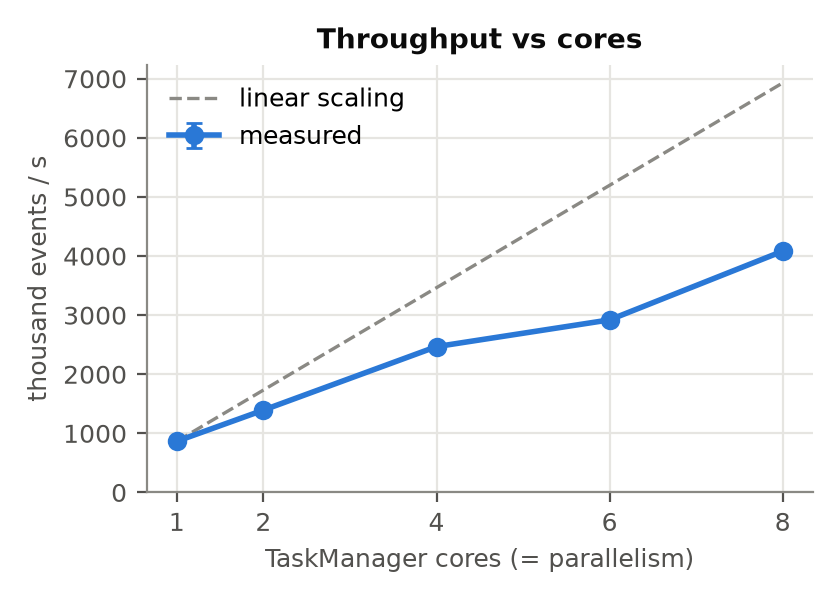
\includegraphics[width=\linewidth]{scalability-throughput}\caption{...}\end{figure}

\subsection{Latency}
% results/figures/latency-vs-rate-c4.png, latency-cdf.png; wait vs processing split; tuning.

\subsection{Long-tail Distribution and Load Balance}
% results/figures/scalability-skew.png (records per parallel instance).

\subsection{Design Trade-off: Out-of-order Bound}
% results/figures/ooo-late.png, ooo-windows.png (real Monday), and results/ooo-synthetic/
% (synthetic input with 2% of trades up to 60 s late, bounds 0 to 120 s).

\section{Smart Visualization}
% docs/dashboard.png: what the trader sees and why it is designed that way.

\section{Conclusion}

\section*{Individual Contributions}
% Each member answers separately:
%  1. The most important decisions you and your group made about the system design.
%  2. The most challenging parts of the design and implementation.
%  3. Your specific contribution, and how you characterize the team's overall functioning.
\subsection*{Name Surname}
\subsection*{Name Surname}

\section*{Use of AI Tools}
% See AI_USE.md. Short disclosure of how AI tools were used in the project and the report.

\bibliographystyle{ACM-Reference-Format}
\bibliography{references}
\end{document}
